\documentclass{article}\usepackage[]{graphicx}\usepackage[]{color}
%% maxwidth is the original width if it is less than linewidth
%% otherwise use linewidth (to make sure the graphics do not exceed the margin)
\makeatletter
\def\maxwidth{ %
  \ifdim\Gin@nat@width>\linewidth
    \linewidth
  \else
    \Gin@nat@width
  \fi
}
\makeatother

\definecolor{fgcolor}{rgb}{0.345, 0.345, 0.345}
\newcommand{\hlnum}[1]{\textcolor[rgb]{0.686,0.059,0.569}{#1}}%
\newcommand{\hlstr}[1]{\textcolor[rgb]{0.192,0.494,0.8}{#1}}%
\newcommand{\hlcom}[1]{\textcolor[rgb]{0.678,0.584,0.686}{\textit{#1}}}%
\newcommand{\hlopt}[1]{\textcolor[rgb]{0,0,0}{#1}}%
\newcommand{\hlstd}[1]{\textcolor[rgb]{0.345,0.345,0.345}{#1}}%
\newcommand{\hlkwa}[1]{\textcolor[rgb]{0.161,0.373,0.58}{\textbf{#1}}}%
\newcommand{\hlkwb}[1]{\textcolor[rgb]{0.69,0.353,0.396}{#1}}%
\newcommand{\hlkwc}[1]{\textcolor[rgb]{0.333,0.667,0.333}{#1}}%
\newcommand{\hlkwd}[1]{\textcolor[rgb]{0.737,0.353,0.396}{\textbf{#1}}}%

\usepackage{framed}
\makeatletter
\newenvironment{kframe}{%
 \def\at@end@of@kframe{}%
 \ifinner\ifhmode%
  \def\at@end@of@kframe{\end{minipage}}%
  \begin{minipage}{\columnwidth}%
 \fi\fi%
 \def\FrameCommand##1{\hskip\@totalleftmargin \hskip-\fboxsep
 \colorbox{shadecolor}{##1}\hskip-\fboxsep
     % There is no \\@totalrightmargin, so:
     \hskip-\linewidth \hskip-\@totalleftmargin \hskip\columnwidth}%
 \MakeFramed {\advance\hsize-\width
   \@totalleftmargin\z@ \linewidth\hsize
   \@setminipage}}%
 {\par\unskip\endMakeFramed%
 \at@end@of@kframe}
\makeatother

\definecolor{shadecolor}{rgb}{.97, .97, .97}
\definecolor{messagecolor}{rgb}{0, 0, 0}
\definecolor{warningcolor}{rgb}{1, 0, 1}
\definecolor{errorcolor}{rgb}{1, 0, 0}
\newenvironment{knitrout}{}{} % an empty environment to be redefined in TeX

\usepackage{alltt}

\usepackage{amsmath}
\usepackage{amsthm}
\usepackage{amsfonts}

\usepackage{hyperref}

\title{Assignment 1 - Solution}
\author{Anh Le}
\IfFileExists{upquote.sty}{\usepackage{upquote}}{}
\begin{document}

\maketitle

Use package \verb`WDI` (an R package that downloads data from the World Bank's World Development Indicators) , download data and plot it. Do not download data by hand, which is both inefficient and not reproducible. Your grader should be able to run your code from start to finish and get the same result.

Here are some ideas to help you start. Feel free to do things you think are cool.
\begin{itemize}
\item Easy: Plot the histogram of countries' GDP / your favorite statistic in one year
\item Easy: Plot the GDP of one country across years
\item Harder: Plot the GDP of multiple countries / continents / groups across years
\item Harder: Add text label, color, etc. to highlight certain countries
\end{itemize}

Make sure to have appropriate title, axis labels, etc.

P/S: There are \href{http://github.com/rOpenGov/psData}{other packages} similar to \verb`WDI` to download Political Science data straight into R. Amazing time that we live in.

\begin{knitrout}
\definecolor{shadecolor}{rgb}{0.969, 0.969, 0.969}\color{fgcolor}\begin{kframe}
\begin{alltt}
\hlkwd{library}\hlstd{(}\hlstr{"WDI"}\hlstd{)} \hlcom{# install.packages as necessary}
\end{alltt}


{\ttfamily\noindent\itshape\color{messagecolor}{\#\# Loading required package: RJSONIO}}\begin{alltt}
\hlkwd{help}\hlstd{(WDI)} \hlcom{# Read the docs -- this one is particularly comprehensible}
\end{alltt}
\end{kframe}
\end{knitrout}

\section{Solution}

\begin{knitrout}
\definecolor{shadecolor}{rgb}{0.969, 0.969, 0.969}\color{fgcolor}\begin{kframe}
\begin{alltt}
\hlcom{## knitr configuration: http://yihui.name/knitr/options#chunk_options}
\hlstd{opts_chunk}\hlopt{$}\hlkwd{set}\hlstd{(}\hlkwc{comment} \hlstd{=} \hlstr{""}\hlstd{,} \hlkwc{error}\hlstd{=} \hlnum{TRUE}\hlstd{,} \hlkwc{warning} \hlstd{=} \hlnum{FALSE}\hlstd{,} \hlkwc{message} \hlstd{=} \hlnum{FALSE}\hlstd{,}
               \hlkwc{tidy} \hlstd{=} \hlnum{TRUE}\hlstd{,} \hlkwc{cache} \hlstd{= F,} \hlkwc{echo} \hlstd{= T,}
               \hlkwc{fig.width} \hlstd{=} \hlnum{5}\hlstd{,} \hlkwc{fig.height} \hlstd{=} \hlnum{5}\hlstd{,} \hlkwc{fig.align}\hlstd{=}\hlstr{"center"}\hlstd{)}
\end{alltt}
\end{kframe}
\end{knitrout}

\begin{knitrout}
\definecolor{shadecolor}{rgb}{0.969, 0.969, 0.969}\color{fgcolor}\begin{kframe}
\begin{alltt}
\hlkwd{rm}\hlstd{(}\hlkwc{list} \hlstd{=} \hlkwd{ls}\hlstd{())}  \hlcom{# Always do this to start with a clean slate}
\hlkwd{library}\hlstd{(}\hlstr{"WDI"}\hlstd{)}
\hlkwd{library}\hlstd{(}\hlstr{"ggplot2"}\hlstd{)}
\hlkwd{library}\hlstd{(}\hlstr{"zoo"}\hlstd{)}  \hlcom{# To deal with time, year, etc.}
\end{alltt}
\end{kframe}
\end{knitrout}

\subsection{US military expenditure}
\begin{knitrout}
\definecolor{shadecolor}{rgb}{0.969, 0.969, 0.969}\color{fgcolor}\begin{kframe}
\begin{alltt}
\hlstd{search_res} \hlkwb{<-} \hlkwd{WDIsearch}\hlstd{(}\hlkwc{string} \hlstd{=} \hlstr{"military"}\hlstd{)}
\hlstd{US_military} \hlkwb{<-} \hlkwd{WDI}\hlstd{(}\hlkwc{country} \hlstd{=} \hlstr{"US"}\hlstd{,} \hlkwc{indicator} \hlstd{=} \hlkwd{c}\hlstd{(}\hlstr{"MS.MIL.XPND.CN"}\hlstd{,} \hlstr{"MS.MIL.XPND.GD.ZS"}\hlstd{),}
    \hlkwc{start} \hlstd{=} \hlnum{1970}\hlstd{,} \hlkwc{end} \hlstd{=} \hlnum{2010}\hlstd{)}
\hlkwd{colnames}\hlstd{(US_military)[}\hlkwd{c}\hlstd{(}\hlnum{4}\hlstd{,} \hlnum{5}\hlstd{)]} \hlkwb{<-} \hlkwd{c}\hlstd{(}\hlstr{"mil_exp"}\hlstd{,} \hlstr{"mil_exp_gdp"}\hlstd{)}  \hlcom{# Rename columns}
\hlstd{US_military} \hlkwb{<-} \hlstd{US_military[}\hlkwd{complete.cases}\hlstd{(US_military), ]}  \hlcom{# Remove missing data}

\hlcom{# Convert column year to Date data type so that R understands that it's a}
\hlcom{# date instead of a number}
\hlstd{US_military}\hlopt{$}\hlstd{year} \hlkwb{<-} \hlkwd{as.Date}\hlstd{(}\hlkwd{strptime}\hlstd{(US_military}\hlopt{$}\hlstd{year,} \hlkwc{format} \hlstd{=} \hlstr{"%Y"}\hlstd{))}

\hlkwd{plot}\hlstd{(US_military}\hlopt{$}\hlstd{year, US_military}\hlopt{$}\hlstd{mil_exp,} \hlkwc{type} \hlstd{=} \hlstr{"l"}\hlstd{,} \hlkwc{xlab} \hlstd{=} \hlstr{"Year"}\hlstd{,} \hlkwc{ylab} \hlstd{=} \hlstr{"Military expenditure (USD)"}\hlstd{,}
    \hlkwc{main} \hlstd{=} \hlstr{"US military expenditure across years"}\hlstd{)}
\hlkwd{abline}\hlstd{(}\hlkwc{v} \hlstd{=} \hlkwd{as.Date}\hlstd{(}\hlstr{"2001"}\hlstd{,} \hlstr{"%Y"}\hlstd{),} \hlkwc{col} \hlstd{=} \hlstr{"red"}\hlstd{)}
\hlkwd{text}\hlstd{(}\hlkwc{x} \hlstd{=} \hlkwd{as.Date}\hlstd{(}\hlstr{"2003"}\hlstd{,} \hlstr{"%Y"}\hlstd{),} \hlkwc{y} \hlstd{=} \hlkwd{quantile}\hlstd{(US_military}\hlopt{$}\hlstd{mil_exp,} \hlkwc{probs} \hlstd{=} \hlnum{0.9}\hlstd{),}
    \hlstr{"Year 2001"}\hlstd{)}
\end{alltt}
\end{kframe}

{\centering 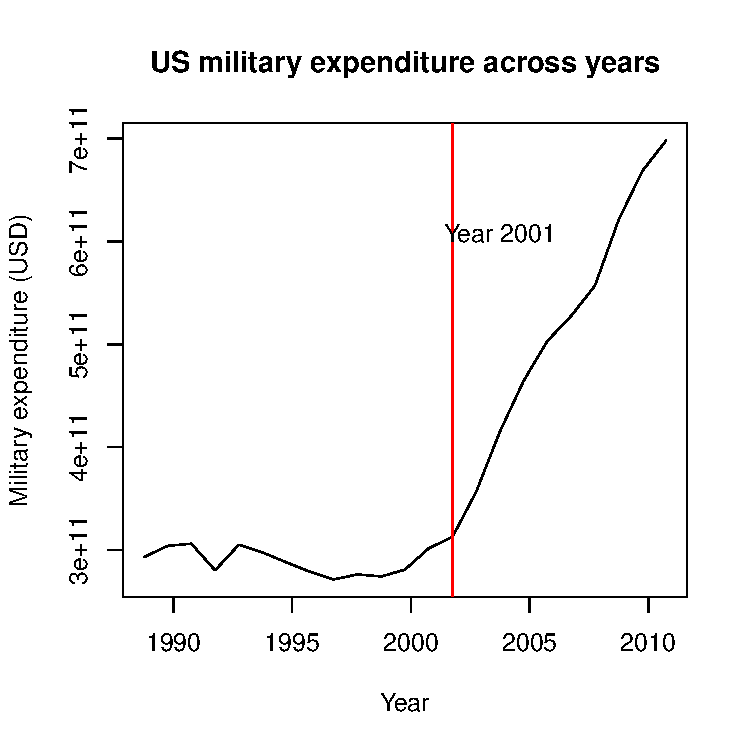
\includegraphics[width=\maxwidth]{figure/US_military_expenditure_plot} 

}



\end{knitrout}

\subsection{World GDP by regions (ggplot2 demonstration)}
\begin{knitrout}
\definecolor{shadecolor}{rgb}{0.969, 0.969, 0.969}\color{fgcolor}\begin{kframe}
\begin{alltt}
\hlkwd{rm}\hlstd{(}\hlkwc{list} \hlstd{=} \hlkwd{ls}\hlstd{())}
\hlstd{world_gdp} \hlkwb{<-} \hlkwd{WDI}\hlstd{(}\hlkwc{country} \hlstd{=} \hlstr{"all"}\hlstd{,} \hlkwc{indicator} \hlstd{=} \hlkwd{c}\hlstd{(}\hlstr{"NY.GDP.PCAP.CD"}\hlstd{),} \hlkwc{extra} \hlstd{=} \hlnum{TRUE}\hlstd{,}
    \hlkwc{start} \hlstd{=} \hlnum{1970}\hlstd{,} \hlkwc{end} \hlstd{=} \hlnum{2010}\hlstd{)}

\hlcom{# Remove aggregate regions (i.e. OECD, etc.)}
\hlstd{world_gdp} \hlkwb{<-} \hlstd{world_gdp[world_gdp}\hlopt{$}\hlstd{region} \hlopt{!=} \hlstr{"Aggregates"}\hlstd{, ]}

\hlcom{# Remove cases with missing data}
\hlstd{world_gdp} \hlkwb{<-} \hlstd{world_gdp[}\hlkwd{complete.cases}\hlstd{(world_gdp), ]}

\hlcom{# as.yearmon is a function in the zoo package, converting string to datetime}
\hlcom{# p is just a common name for a plot object}
\hlstd{p} \hlkwb{<-} \hlkwd{ggplot}\hlstd{(}\hlkwc{data} \hlstd{= world_gdp,} \hlkwd{aes}\hlstd{(}\hlkwc{x} \hlstd{=} \hlkwd{as.Date}\hlstd{(}\hlkwd{as.yearmon}\hlstd{(year)),} \hlkwc{y} \hlstd{= NY.GDP.PCAP.CD))} \hlopt{+}
    \hlkwd{labs}\hlstd{(}\hlkwc{x} \hlstd{=} \hlstr{"Year"}\hlstd{,} \hlkwc{y} \hlstd{=} \hlstr{"GDP per capita (current USD)"}\hlstd{)}

\hlstd{p_all_countries} \hlkwb{<-} \hlstd{p} \hlopt{+} \hlkwd{geom_line}\hlstd{(}\hlkwd{aes}\hlstd{(}\hlkwc{group} \hlstd{= country,} \hlkwc{color} \hlstd{= region))}
\hlstd{p_all_countries}
\end{alltt}
\end{kframe}

{\centering 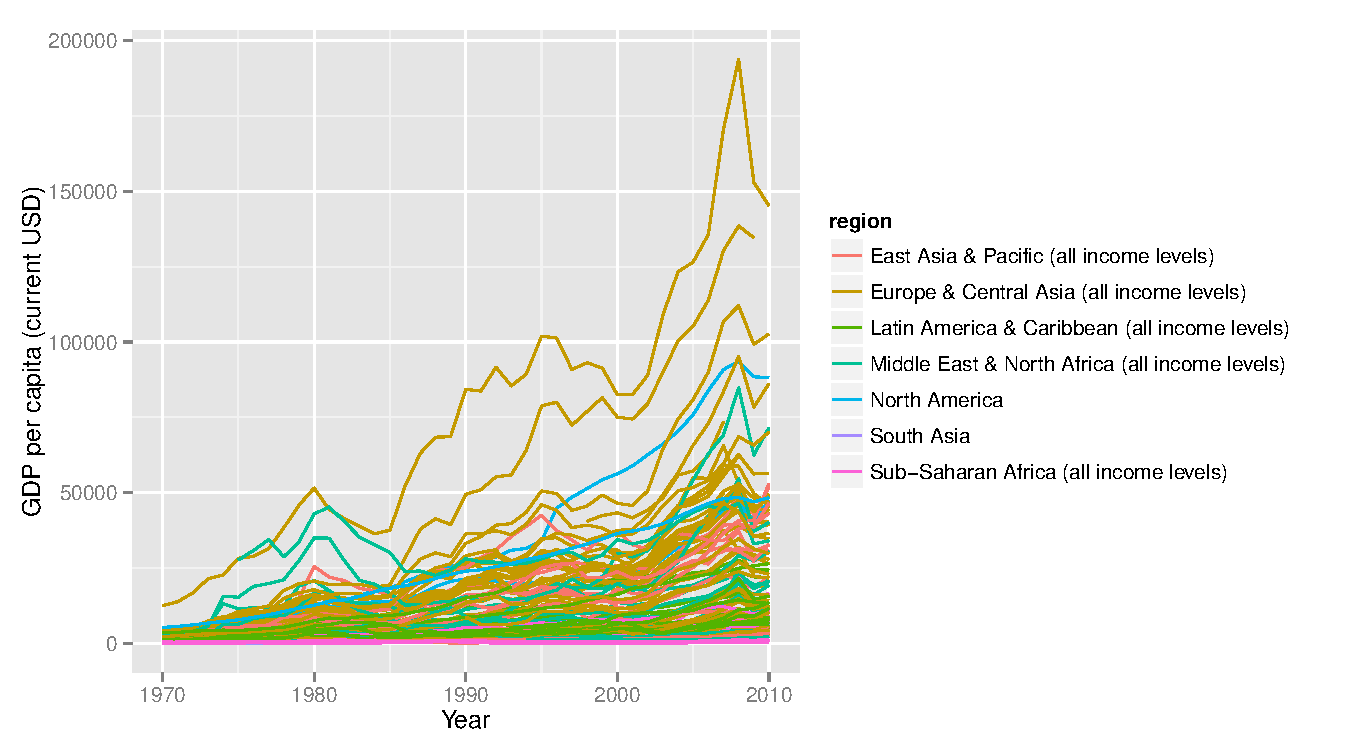
\includegraphics[width=\maxwidth]{figure/unnamed-chunk-3} 

}



\end{knitrout}

Hmm, despite all the talk about China and East Asian miracles, the countries who saw the strongest growth is in Europe \& Central Asia. I wonder what those countries are?

\begin{knitrout}
\definecolor{shadecolor}{rgb}{0.969, 0.969, 0.969}\color{fgcolor}\begin{kframe}
\begin{alltt}
\hlcom{# Select only the rows where the year is 2009}
\hlstd{world_gdp_2009} \hlkwb{<-} \hlstd{world_gdp[world_gdp}\hlopt{$}\hlstd{year} \hlopt{==} \hlnum{2009}\hlstd{, ]}

\hlcom{# Select only the rows where its GDP per cap is in the top 5 percent}
\hlstd{world_gdp_2009_top_5_percent} \hlkwb{<-} \hlstd{world_gdp_2009[world_gdp_2009}\hlopt{$}\hlstd{NY.GDP.PCAP.CD} \hlopt{>=}
    \hlkwd{quantile}\hlstd{(world_gdp_2009}\hlopt{$}\hlstd{NY.GDP.PCAP.CD,} \hlnum{0.95}\hlstd{), ]}

\hlcom{# geom_text() will add text to the plot. In this case, the text label is}
\hlcom{# country name}
\hlstd{p_rich_countries} \hlkwb{<-} \hlstd{p_all_countries} \hlopt{+} \hlkwd{geom_text}\hlstd{(}\hlkwc{data} \hlstd{= world_gdp_2009_top_5_percent,}
    \hlkwd{aes}\hlstd{(}\hlkwc{x} \hlstd{=} \hlkwd{as.Date}\hlstd{(}\hlstr{"2009"}\hlstd{,} \hlstr{"%Y"}\hlstd{),} \hlkwc{y} \hlstd{= NY.GDP.PCAP.CD,} \hlkwc{label} \hlstd{= country))}
\hlstd{p_rich_countries}
\end{alltt}
\end{kframe}

{\centering 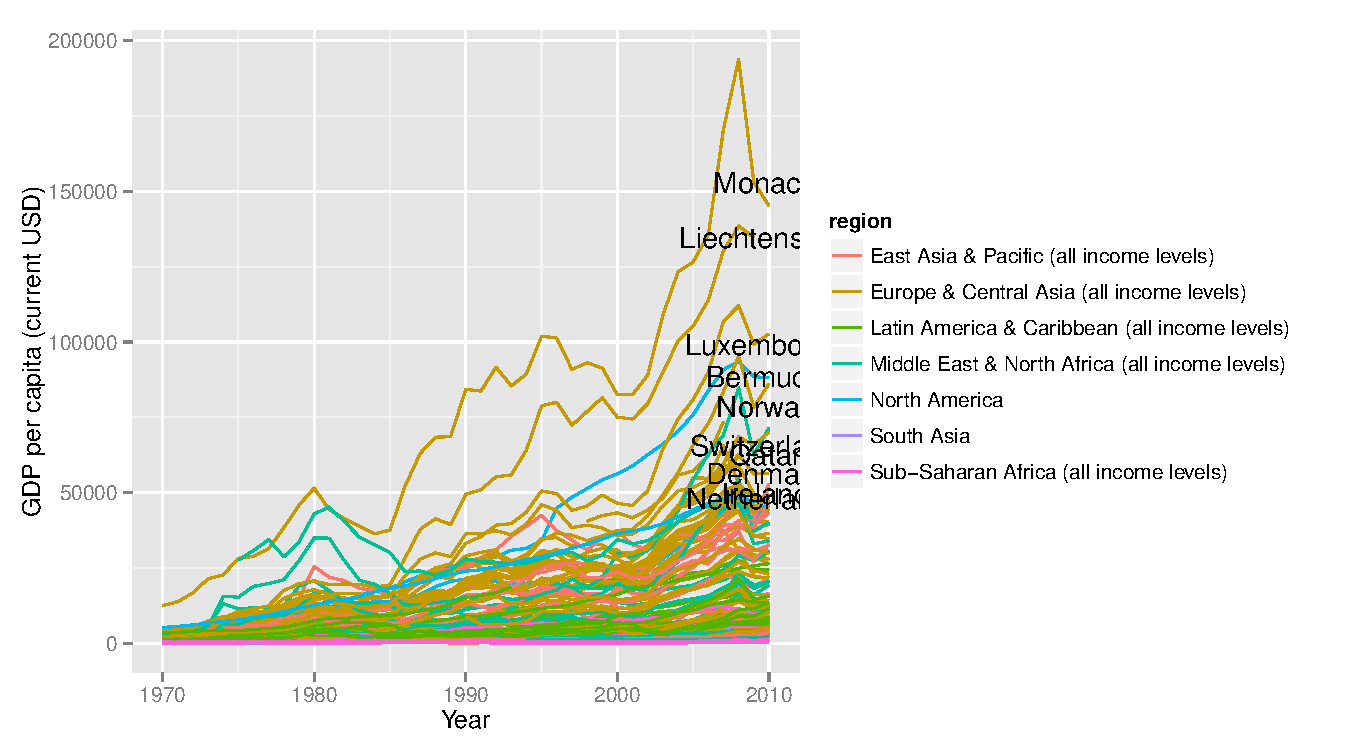
\includegraphics[width=\maxwidth]{figure/unnamed-chunk-4} 

}



\end{knitrout}

Let's see where are the East Asian miracles in the plot. US for scale.

\begin{knitrout}
\definecolor{shadecolor}{rgb}{0.969, 0.969, 0.969}\color{fgcolor}\begin{kframe}
\begin{alltt}
\hlstd{world_gdp_select} \hlkwb{<-} \hlstd{world_gdp[world_gdp}\hlopt{$}\hlstd{country} \hlopt \hlkwd{c}\hlstd{(}\hlstr{"China"}\hlstd{,} \hlstr{"Japan"}\hlstd{,} \hlstr{"Korea, Rep."}\hlstd{,}
    \hlstr{"United States"}\hlstd{), ]}

\hlcom{# I blur the countries' line with alpha = 0.25 Then I add geom_line() and}
\hlcom{# geom_text() for the selected countries}
\hlstd{p} \hlopt{+} \hlkwd{geom_line}\hlstd{(}\hlkwd{aes}\hlstd{(}\hlkwc{group} \hlstd{= country,} \hlkwc{color} \hlstd{= region),} \hlkwc{alpha} \hlstd{=} \hlnum{0.25}\hlstd{)} \hlopt{+} \hlkwd{geom_line}\hlstd{(}\hlkwc{data} \hlstd{= world_gdp_select,}
    \hlkwd{aes}\hlstd{(}\hlkwc{group} \hlstd{= country),} \hlkwc{size} \hlstd{=} \hlnum{1}\hlstd{)} \hlopt{+} \hlkwd{geom_text}\hlstd{(}\hlkwc{data} \hlstd{= world_gdp_select[world_gdp_select}\hlopt{$}\hlstd{year} \hlopt{==}
    \hlnum{2010}\hlstd{, ],} \hlkwd{aes}\hlstd{(}\hlkwc{x} \hlstd{=} \hlkwd{as.Date}\hlstd{(}\hlstr{"2009"}\hlstd{,} \hlstr{"%Y"}\hlstd{),} \hlkwc{y} \hlstd{= NY.GDP.PCAP.CD,} \hlkwc{label} \hlstd{= country))}
\end{alltt}
\end{kframe}

{\centering 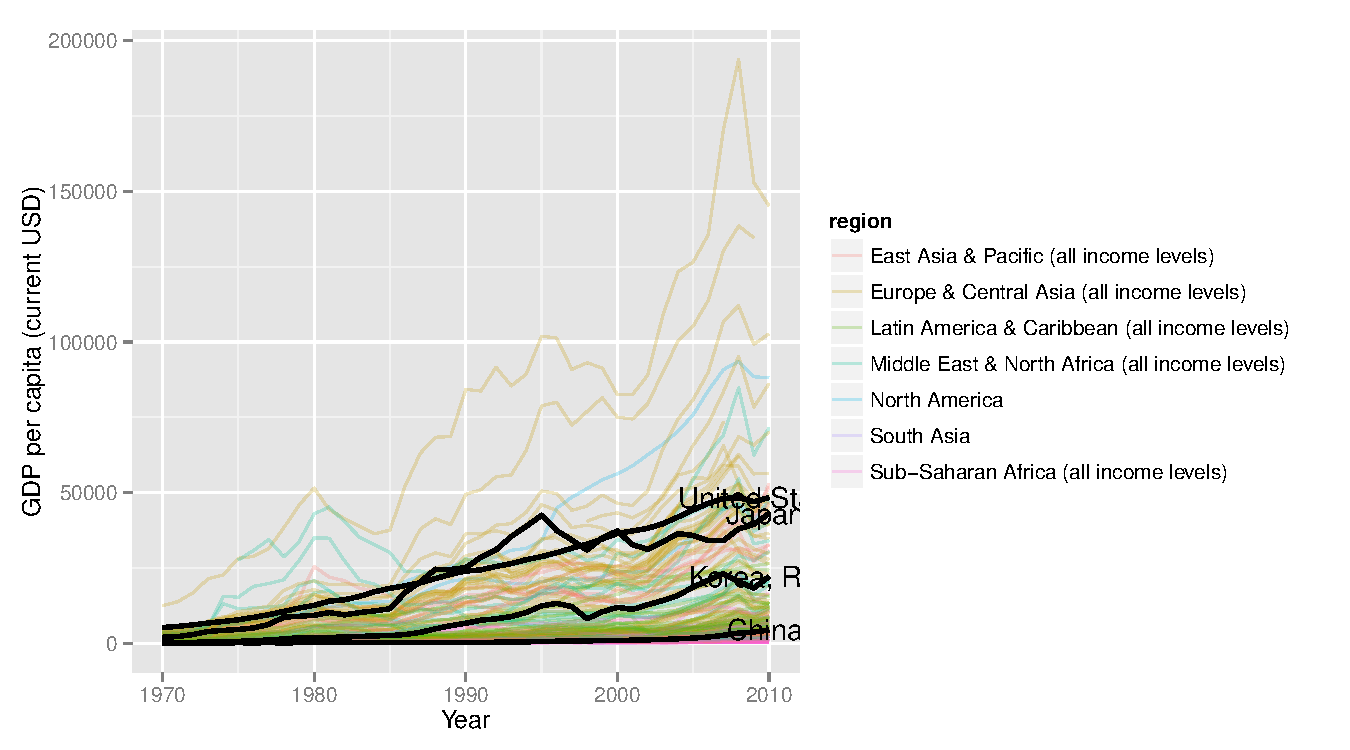
\includegraphics[width=\maxwidth]{figure/unnamed-chunk-5} 

}



\end{knitrout}

\end{document}
